\section{Background}

\begin{figure*}[h!]
	\begin{subfigure}{.53\textwidth}
		\centering
		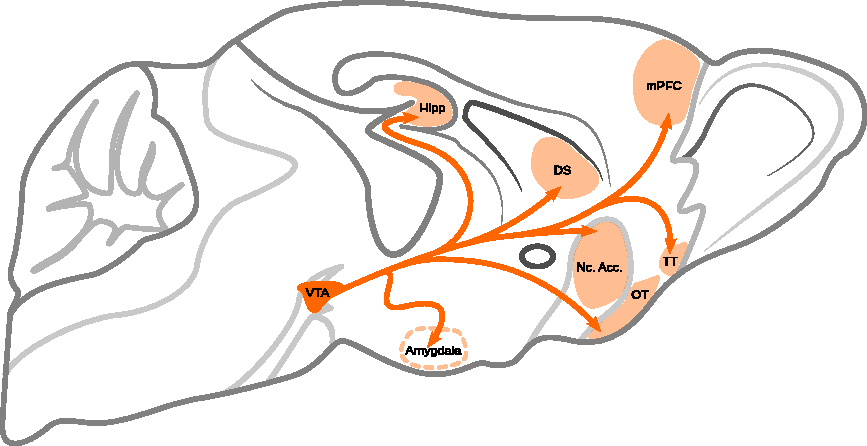
\includegraphics[width=\textwidth]{img/model_literature}
		\caption{
			Literature-based schematic map of VTA dopaminergic projections \cite{Aransay2015,Fields2007,Ikemoto2007,Hnasko2012,Pan2010}.
			Dotted structures are off-slice, and projection arrows do not reflect fiber bundle paths.
			Abbreviations: Hipp (Hippocampus), DS (Dorsal Striatum), NAcc (Nucleus Accumbens), OT (Olfactory Tuberculum), mPFC (medial Prefrontal Cortex), TT (Tenia Tecta).
			}
		\label{fig:ml}
	\end{subfigure}
	\begin{subfigure}{.45\textwidth}
		\centering
		\vspace{-1em}
		%\includegraphics[width=\textwidth]{data/model_dopaminergic}
		\includedot[width=1.1\textwidth]{data/network_model}
		\vspace{-0.95em}
		\caption{
			Simplified network model of 1-step signal transduction following optogenetic stimulation of the VTA.
			The $\mathrm{u_1}$ weighting corresponds to VTA somatic excitability and $\mathrm{u_{2a},u_{2b},u_{2c}}$ and $\mathrm{u_{2d}}$ correspond to transmission at the dopaminergic synapses in the respective projection areas.
			}
		\label{fig:md}
	\end{subfigure}
	\begin{subfigure}{.96\textwidth}
		\centering
		\missingfigure[figwidth=0.40\textwidth]{dopaminergic cell schematic}
		\caption{
			Schematic overview of a dopaminergic neuron, which can be applied to model all cells in the nucleus.
			Due to the projection distance and the manifold projection areas the soma is located in the VTA, and the synapses in one or multiple other voxels in the projection areas.
			}
		\label{fig:nm}
	\end{subfigure}
	\caption{
		\textbf{The cell biological compartmentalization of dopaminergic neurotransmission (and susceptibility to psychopharmacology) can partly be mapped onto neuroanatomical features by a simple network model.}
		Depicted are schematic overviews of the VTA dopaminergic system at various spatial resolutions.
		}
	\label{fig:m}
\end{figure*}

The ultimate assessment standard for knowledge is its ability to inform action.
As such, neuroscience incrementally aims to support the development of meaningful and predictable control of the brain.
Within this endeavour, it is the most easily accessible components of the brain, given current technology, which can provide the greatest opportunities for advancement.

The dopaminergic system is an evolutionarily well-conserved \cite{Yamamoto2011}, strongly localized, and widely projecting set of neurons \cite{Aransay2015,Fields2007,Ikemoto2007,Hnasko2012}.
On account of the small number of neurons, tractography commonly fails to resolve the degree centrality of such nodes, yet it is precisely the small number of widely branching and closely similar neurons, which makes the dopaminergic system a credible candidate for truly node-like function in coordinating brain activity.
As is expected given such salient features, the system is widely implicated in neuropsychiatric phenomena (including
addiction \cite{DiChiara1988,DiChiara1999},
attentional control \cite{Nieoullon2002},
motivation \cite{Salamone1994},
creativity \cite{Chermahini2010},
personality \cite{Depue1999},
neurodegeneration \cite{Masliah2000},
and schizophrenia \cite{Howes2009}),
and is a common target for pharmacological interventions.
Manipulation of the dopaminergic system extends widely beyond the medical field, and includes performance-enhancing \cite{Mehta2000,Turner2003}, as well as recreational usage \cite{DiChiara1988}.
As such, better and more predictively powerful models of the dopaminergic system can enhance numerous aspects of human activity, in the clinic and beyond.

Neuroscience experimentation in human subjects is methodologically constrained, and consequently at a strong competitive disadvantage of offering cell biological insights.
Due to the high evolutionary conservation of the dopaminergic system, however, it is an excellent candidate for translational study.
Of the common model animals, the mouse offers advantages not only absent from higher primates, but from most other model animals in general.
These include short generation spans, broad availability of transgenic lines, highly accessible histology, and the most compact size among mammalian model organism brains.
Far from trivial, this latter trait offers a significant advantage for numerous imaging techniques, including optics, optoacoustics, and even magnetic resonance imaging (MRI).
Furthermore, the small size greatly increases experiment scalability and multi-center reproducibility.
Particularly concerning pharmacological research, the mouse additionally possesses a high metabolic rate, allowing for rapid drug clearing and thus high contrast in repeated drug administrations.

The brain is a holistically functioning organ, coordinating perception, decision, and action, moreso than scale-invariant metabolic phenomena.
Consequently, localized study of the brain only offers limited insight into the mechanism, just as localized control of the brain can only offer very limited control over its function.
This consideration not only supports the endeavour to study widely projecting neurotransmitter systems, but also suggests that whole-brain measurement techniques are uniquely suited to describe them.
Owing to its deep penetration, high rostrocaudal coverage, and large-scale usage in human studies, functional MRI (fMRI) is on of the foremost methods for studying the function of the dopaminergic system.

In order to increase the signal to noise ratio (SNR) of a neurotransmitter system encompassing a small number of cells, stimulation is a common requirement.
While the localization of widely projecting dopaminergic cells into nuclei makes the targeting of this system comparatively easy, dopaminergic nuclei also contain notable populations of non-dopaminergic cells, with different functions and different pharmacological susceptibilities \cite{Taylor2014}.
In order to specifically target dopaminergic cells, these need to be sensitized to an otherwise inert stimulus in a transcription-dependent manner.
One method of achieving this is via optogenetics (light-stimulation of cells expressing a light-sensitive transmembrane protein \cite{Boyden2005}), where the optogenetic construct is expressed Cre-conditionally \cite{Orban1992} in a transgenic animal expressing Cre-recombinase under a dopaminergic promoter.
Thu application of this combination of methods to fMRI is commonly referred to as opto-fMRI, and enjoys great popularity \cite{Desai2011,Grandjean2019} --- affording a significant potential for technology transfer of novel assay applications.

In developing a powerful new assay which optimally ties in all of the aforementioned characteristics, it is most appropriate to select a stimulation site for the entire dopaminergic system.
While the dopaminergic system is centralized in the midbrain, it consists not of one, but of two pairs of lateralized nuclei, the Ventral Tegmental Area (VTA), and Substantia Nigra pars compacta (SNc).
Of these, the VTA has the broader efferent distribution, whereas the SNc projects primarily to the dorsal striatum \cite{Pan2010}.

The most popular means of producing spatially resolved sensitivity summaries from fMRI, and opto-fMRI in particular, is the general linear modelling (GLM) of stimulus evoked activity \cite{Friston1995}.
In this procedure, a precisely specified stimulus train is presented to the brain (in opto-fMRI, directly, without mediation via sensory neurons).
The analysis is performed by convolving the stimulus train with an impulse response function (IRF), and performing a mass univariate regression analysis --- across all voxels.
While powerful, this approach is also strongly limiting, since it implies that all voxels in the brain are exposed in an indistinguishable fashion to the stimulation.
Particularly in cases where stimulation is introduced via well-known pathways, a simple network model of signal transduction can easily be implemented via seed-based connectivity (\cref{fig:nm}).
Additionally, in the case of neurotransmitter systems with colocalized cell bodies and long efferent projections, the macroscopic resolution of fMRI can be used to distinguish cell biological processes (e.g. excitability at the soma and signal transmission to the postsynaptic membrane).

To enable the whole-brain modelling of human VTA dopaminergic function in mice, a number of novel results need to be produced.
A proof-of-principle study needs to be conducted to assess the feasibility of the methods in the model animal.
The study design needs to include controlled but significant methodological variation, in order to lay a reliable and well-informed foundation for the technique. 
Given a positive outcome, the variation in the results needs to be described and evaluated, in order to lay the foundation for assay reproduction and refinement.
Finally, a voxelwise summary of baseline dopaminergic function needs to be published in a standard volumetric space, to easily enable co-registration and result integration or comparison.
